\section{Derived data}

\begin{frame}{Example 3: produce once, analyse many times}
 \small
 {\centering
 \begin{tikzpicture}[node distance=6mm,every node/.style={align=center,font=\footnotesize},box/.style={draw=blue!60,fill=blue!5,rounded corners,minimum height=10mm}]
 \node[box] (raw) {Raw AO2D};
 \node[box,right=of raw] (prod) {Femto producer};
 \node[box,right=of prod] (derived) {Derived files\\kinematics + masks};
 \node[box,below=8mm of derived,draw=teal,fill=teal!8] (d2d) {Derived-to-derived producer\\\textbf{optional}};
 \draw[->,thick] (raw)--(prod);
 \draw[->,thick] (prod)--(derived);
 \draw[->,thick] (derived)--(d2d);
 \draw[->,thick,teal] (d2d.east) to[out=0,in=0,looseness=2.5] node[right,font=\scriptsize] {repeat} (derived.east);
 \node[box,left=12mm of d2d] (pairs) {Collision tagger\\+ pair task};
 \draw[->,thick] (derived.south west)--(pairs.north east);
 \draw[->,thick] (d2d)--(pairs);
 \end{tikzpicture}\par}
 \medskip
 \begin{itemize}
 \item Producer-only workflow: raw AO2D dependencies, without QA or pairing.
 \item Standalone analysis: the derived tables already contain the required information.
 \item The optional derived-to-derived producer can run repeatedly on the derived files, refining the stored sample.
 \end{itemize}
 \src{O2Physics/PWGCF/Femto/TableProducer/femtoProducer.cxx; O2Physics/PWGCF/Femto/DataModel/FemtoTables.h}
\end{frame}

\begin{frame}[fragile]{Derived production: explicitly enable the output tables}
 \begin{lstlisting}
"CollisionTables": {
  "produceCollisions": "1", "produceCollisionMasks": "1"
},
"TrackTables": {
  "produceTracks": "1", "produceTrackMasks": "1"
},
"V0Tables": {
  "produceLambdas": "1", "produceLambdaMasks": "1"
}
 \end{lstlisting}
 \begin{itemize}
 \item \texttt{"-1"}: auto-enable from downstream task subscriptions in a full workflow.
 \item \texttt{"1"}: force on for a producer-only derived-data production; \texttt{"0"}: force off.
 \item Only kinematics and masks are stored: the QA tasks cannot run on this derived dataset.
 \end{itemize}
 \note{Additional extra-observable tables could be stored to enable QA, but they are intentionally omitted from this compact example. All unrelated table switches are explicitly off in producer.json. Do not delete daughter-only track rows: Lambda daughter references must remain valid for the cleaner and CPR. Keep AnalysisResults.root with the producer configuration/selection metadata alongside the derived file; the minimal six-table output does not contain detector observables or that histogram metadata.}
 \src{O2Physics/PWGCF/Femto/Core/trackBuilder.h; O2Physics/PWGCF/Femto/Core/v0Builder.h; O2Physics/PWGCF/Femto/Core/collisionBuilder.h}
\end{frame}

\begin{frame}[fragile]{Derived production: the writer selects what reaches disk}
 \begin{lstlisting}
{
  "OutputDirector": {
    "resfile": "FemtoDerived", "resfilemode": "RECREATE",
    "OutputDescriptors": [
      {"table": "AOD/FCOL/1"}, {"table": "AOD/FCOLMASK/1"},
      {"table": "AOD/FTRACK/1"}, {"table": "AOD/FTRACKMASK/1"},
      {"table": "AOD/FLAMBDA/1"}, {"table": "AOD/FLAMBDAMASK/2"}
    ]
  }
}
 \end{lstlisting}
 \small \texttt{--aod-writer-json writer.json} activates this output selection.\par\medskip
 \texttt{examples/03-derived-data/produce.sh} runs the producer and its raw-AO2D dependencies.\par\medskip
 Two outputs: \texttt{FemtoDerived.root} (tables) and \texttt{AnalysisResults.root} (producer metadata).
 \note{The table descriptor includes origin, description and version; these match the local FemtoTables.h. The writer configuration is separate from DPL task configuration. The default one-timeframe-per-output-DF behavior is retained. OutputDirector ntfmerge is intentionally omitted: unlike task configurable values, its JSON parser requires a numeric JSON value.}
 \src{O2Physics/PWGCF/Femto/DataModel/FemtoTables.h; O2/Framework/Core/src/DataOutputDirector.cxx}
\end{frame}

\begin{frame}{Hyperloop: producer wagon and derived-data output}
 \centering
 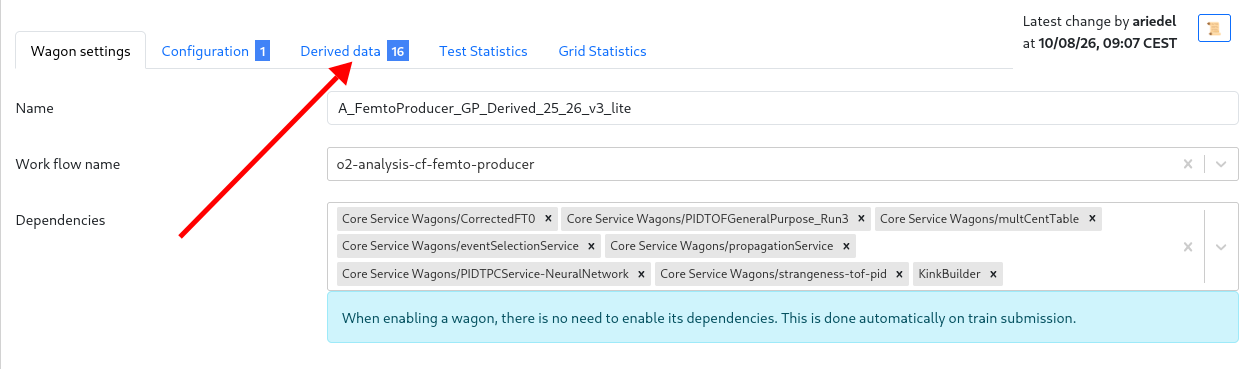
\includegraphics[width=\textwidth,height=.66\textheight,keepaspectratio]{slides/assets/hyperloop-producer-wagon.png}
 \par\medskip
 \small The producer wagon's \textbf{Derived data} tab configures which output tables are written.
 \note{User-provided screenshot. The dependency list shown belongs to this example wagon and includes additional species beyond the proton-Lambda tutorial. Hyperloop automatically includes configured dependencies on train submission, as indicated in the UI.}
 \src{O2Physics/PWGCF/Femto/TableProducer/femtoProducer.cxx}
\end{frame}

\begin{frame}{Hyperloop: select the derived tables}
 \centering
 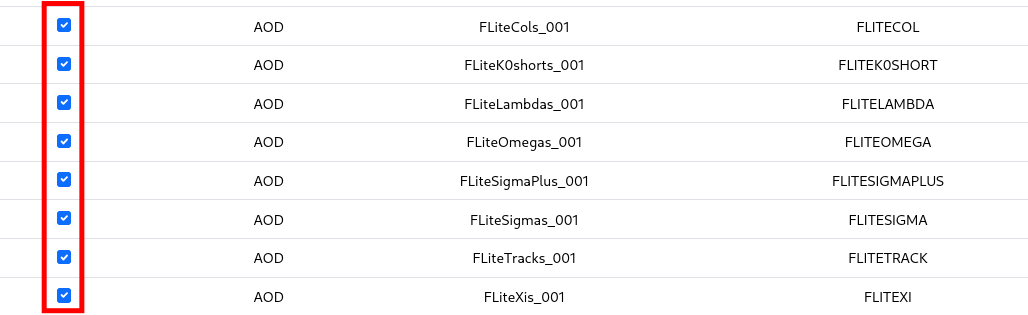
\includegraphics[width=\textwidth,height=.66\textheight,keepaspectratio]{slides/assets/hyperloop-derived-tables.png}
 \par\medskip
 \small Select the tables to write; a Lite-table production is shown here.
 \note{User-provided screenshot illustrating table checkboxes. This screenshot contains multiple Lite species; the local tutorial instead writes the full-kinematic collision, track and Lambda tables with their masks. Select the table set appropriate to the production and downstream consumers; do not treat the screenshot as the exact six-table tutorial selection.}
 \src{O2Physics/PWGCF/Femto/DataModel/FemtoTables.h}
\end{frame}

\begin{frame}{Hyperloop: force the selected producer tables on}
 \centering
 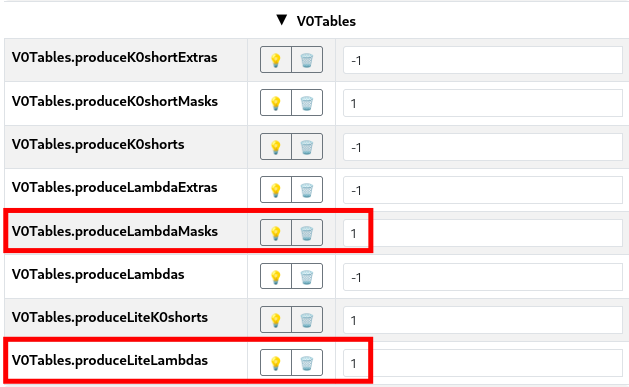
\includegraphics[width=.78\textwidth,height=.70\textheight,keepaspectratio]{slides/assets/hyperloop-producer-table-flags.png}
 \par\smallskip
 \small Selected output tables must also be produced: set their producer switches to \texttt{1}.
 \note{User-provided screenshot of V0Tables. The highlighted example forces Lambda masks and Lite Lambdas on. Auto mode -1 follows downstream subscriptions; for producer-only output, explicitly enabling the intended tables avoids depending on consumer task subscriptions. Writer selection and producer table enablement are separate settings.}
 \src{O2Physics/PWGCF/Femto/Core/v0Builder.h}
\end{frame}

\begin{frame}[fragile]{Standalone pairing on derived data}
 \small
 \begin{lstlisting}[language=bash]
# examples/03-derived-data/analyze.sh
# input_derived.txt contains: FemtoDerived.root
Options=(-b --configuration json://pair.json
         --aod-file @input_derived.txt)
o2-analysis-cf-femto-producer-collision-tagger "${Options[@]}" |
  o2-analysis-cf-femto-pair-track-v0 "${Options[@]}" --run
 \end{lstlisting}
 \begin{itemize}
 \item The same \texttt{TrackSelection1}, \texttt{LambdaSelection1}, mixing and pair settings.
 \item Collision tagging is included from the start and recomputed for the current pair wagon.
 \item Raw-AO2D event-selection, propagation and PID services are no longer needed.
 \end{itemize}
 \small Local: derived input list + \texttt{pair.json}.\par
 Hyperloop: derived dataset + tagger and pair wagons; matching table versions.
 \src{O2Physics/PWGCF/Femto/Tasks/femtoPairTrackV0.cxx; O2Physics/PWGCF/Femto/TableProducer/femtoProducerCollisionTagger.cxx}
\end{frame}

\begin{frame}[fragile]{Local dataframe sizes: \texttt{o2-aod-merger}}
 \begin{lstlisting}[language=bash]
o2-aod-merger --input input_derived.txt \
  --output FemtoMerged.root --max-size 100000000
 \end{lstlisting}
 \begin{itemize}
 \item Input: a text list of compatible, self-contained derived ROOT files.
 \item Combines complete input dataframes into larger output \texttt{DF\_...} directories and updates table indices.
 \item \texttt{--max-size}: approximate target size of an uncompressed dataframe directory, in bytes; it is not a ROOT file-size limit.
 \item Larger dataframes can provide more mixing partners; they also require more memory.
 \end{itemize}
 \begin{block}{Boundary of the operation}
 An existing large dataframe is not split into smaller ones. \texttt{--max-size 0} preserves input dataframe boundaries (needed for non-self-contained inputs).
 \end{block}
 \note{The size is tested after copying a whole input DF, so the target can be exceeded. Do not use hadd for AOD tables with row-index references. The example merge.sh refuses to overwrite an existing output. No merger is needed to combine histogram-only AnalysisResults.root files.}
 \src{O2/Framework/AODMerger/src/aodMerger.cxx}
\end{frame}
